\documentclass[sigconf]{acmart}

\usepackage{graphicx}

\setcopyright{none}
\settopmatter{printacmref=false} % Removes citation information below abstract
\renewcommand\footnotetextcopyrightpermission[1]{} % removes footnote with conference information in first column
\pagestyle{plain} % removes running headers
\begin{document}
\title{Balancing the trade-off between accuracy and interpretability in software defect prediction, ESE 2019}
\author{Rahul Yedida}
\affiliation{Department of Computer Science, NC State University}
\email{ryedida@ncsu.edu}

\begin{abstract}
Can we build accurate ML systems that are also interpretable? This poster summarizes the method described in \cite{mori2019balancing}: a novel classification model is proposed that is both accurate and interpretable. It extends the standard Naive Bayes model to create an ensemble, and then creates a linear approximation. The method, superposed Naive Bayes (SNB) produces a balanced output that is both interpretable and accurate, and its results are discussed in the context of software datasets.
\end{abstract}

\maketitle
\footnotetext{Toshiki Mori and Naoshi Uchihira. Balancing the trade-off between accuracy and interpretability in software defect prediction. Empirical Software Engineering, 24(2):779–825, 2019.}
\section{Introduction}
Recently, interpretability is becoming more important in machine learning \cite{Ribeiro2016} in several domains including healthcare, where computational models cannot be blindly trusted without clear reasoning behind decisions. However, it has been observed that there is in general a trade-off between interpretability of models and accuracy, and the proper balance may be different in each domain.

Software engineering is one of the domains where machine learning could potentially be useful. Among other use cases, machine learning techniques have been extensively applied in software defect prediction \cite{malhotra2015systematic}. This paper outlines a novel classification model that first builds an ensemble of Naive Bayes classifiers and then creates a linear approximation, with the intention that the first step improves accuracy, and the second step improves interpretability.

We aim to answer the following research questions:
\begin{enumerate}
	\item \textbf{How accurate are the current predictors?} To compare the accuracy of SNB with other classifiers, we use multiple k-fold cross-validation and a double Scott-Knott test \cite{jelihovschi2014scottknott}.
	\item \textbf{How do we assess the interpretability of classifiers?} We use a qualitative assessment based on \cite{lipton2016mythos}, which is comprised of model transparency, component transparency, and algorithmic transparency.
	\item \textbf{How can we balance the trade-off between accuracy and interpretability?} To analyze this, we combine the results measuring accuracy and interpretability. Our findings confirm the general assumption that there is a trade-off between the two; nevertheless, SNB gives balanced outputs that satisfy both criteria.
\end{enumerate}

\section{Method}
We focus on binary classification problems, since multi-class classification problems can be converted to binary classification problems by schemes such as one-vs-rest.

\subsection{Naive Bayes}
Naive Bayes is a special case of Gaussian Discriminant Analysis with the stronger assumption that the predictor variables are conditionally independent given the target variable. We then use Bayes' rule to compute posterior likelihoods:

\begin{equation}
p(y=1|x_1,\ldots,x_d) \propto p(y=1)\prod\limits_{i=1}^d p(x_i|y=1)
\label{eq:1}
\end{equation}

From this, we compute the log-odds ratio:

\begin{equation}
\frac{\log p(y=1|x_1,\ldots,x_d)}{\log p(y=0|x_1,\ldots,x_d)} = \log \frac{p(y=1)}{p(y=0)} + \sum\limits_{i=1}^d \log \frac{p(x_i|y=1)}{p(x_i|y=0)}
\label{eq:2}
\end{equation}

which can be expressed as

\begin{equation}
W(X) = W_0 + \sum W_i(x_i)
\label{eq:3}
\end{equation}

Each term here is called a weight of evidence. A positive $W_i(x_i)$ indicates that the state of $x_i$ is evidence in favor of the hypothesis that $y=1$. The total sum of the weights of evidence gives a raw score $W(X)$, a higher value indicating a higher posterior likelihood that $y=1$.

There are some issues with the standard Naive Bayes. First is the issue of cases where a dependent variable value and an independent variable value never occur, resulting in an indefinite weight of evidence. This can be fixed by adding a small sample correction to all likelihoods. This is called Laplace smoothing. The second issue is with numeric values. This can be solved by assuming a prior distribution on that independent variable and using it in the posterior likelihood expression. The third issue is with post-processing of the raw score. Class membership probability estimates can be obtained by sigmoid calibration of the raw scores:

\begin{equation}
p_{nb}(X) = \sigma(c_0 + c_1 W(X)) = \frac{1}{1 + \exp(-(c_0 + c_1 W(X)))}
\label{eq:4}
\end{equation}

Given a discrimination threshold $t$, we predict $C_{nb}(X|t) = 1$ if $p_{nb}(X) \geq t$.

\subsection{Naive Bayes ensemble}
Creating ensembles can be done in several ways involving random selection of feature subsets to train different models. Boosting is one such technique that incrementally builds an ensemble by reweighting each training sample; correctly classified samples are given a lower weight, and incorrectly classified samples are given a higher weight. AdaBoost \cite{freund1997decision} uses a multiplicative weight update rule. An extension of this called stochastic gradient boosting uses a gradient descent approach at each iteration.

\begin{figure}
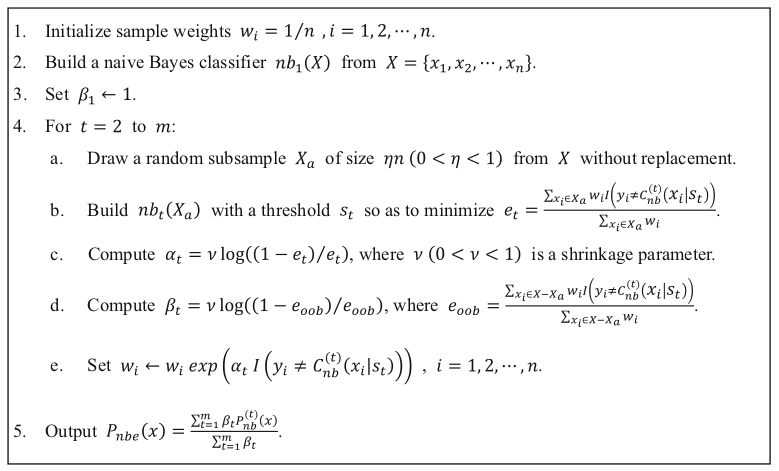
\includegraphics[width=0.45\textwidth]{fig1.png}
\caption{Naive Bayes ensemble algorithm}
\label{fig:1}
\end{figure}

Figure \ref{fig:1} shows the algorithm to create a Naive Bayes ensemble.

\subsection{Superposed Naive Bayes}
We then create a single Naive Bayes model by superposing the different models, weighted by the weights of evidence. Figure \ref{fig:2} shows an example.

\begin{figure}
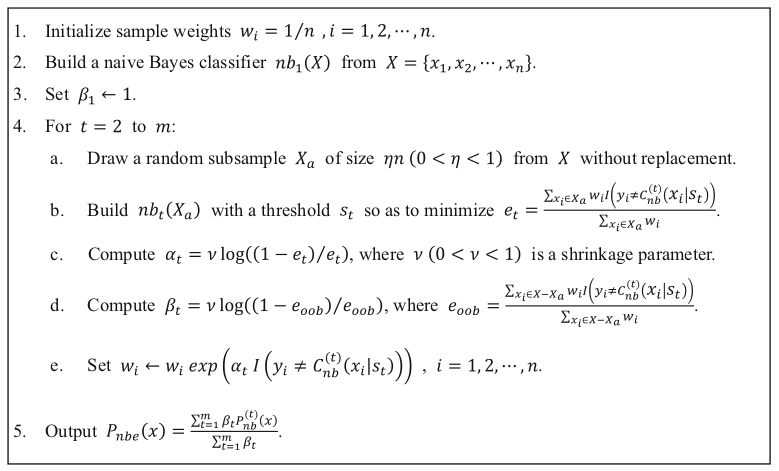
\includegraphics[width=0.45\textwidth]{fig1.png}
\caption{Superposing Naive Bayes ensemble}
\label{fig:2}
\end{figure}

From \eqref{eq:3} and \eqref{eq:4}, the output of the Naive Bayes ensemble is

\begin{equation}
p_{nbe}(X) = \frac{\sum\limits_{t=1}^m \beta_t p_{nb}^{(t)}(X)}{\sum\limits_{t=1}^m \beta_t} = \frac{\sum\limits_{t=1}^m \beta_t \sigma\left(c_0^{(t)} + c_1^{(t)} \sum\limits_{i=0}^d W_i^{(t)}(x_i)\right)}{\sum\limits_{t=1}^m \beta_t}
\label{eq:5}
\end{equation}

We now approximate the sigmoid function by its first order Taylor series approximation about $c_0$:

\begin{align}
	\sigma\left(c_0^{(t)} + c_1^{(t)} W^{(t)}(X)\right) &= \sum\limits_{n=0}^\infty \frac{\sigma^{(n)}(c_0^{(t)}}{n!}\left(c_1^{(t)}W^{(t)}(X)\right) \nonumber \\ &\approx \sigma(c_0^{(t)}) + \left( c_1^{(t)} \sigma(c_0^{(t)}) \left( 1 - \sigma(c_0^{(t)}) \right) \right) W^{(t)}(X)
\end{align}

which is of the form $a_t + b_t W^{(t)}(X)$.

\section{Experimental Settings}
We use 13 datasets from two sources: a cleaned version of the NASA MDP datasets provided by \cite{shepperd2013data}, and the JIT datasets provided by \cite{kamei2012large}. From the first source, 11 datasets that were initially from various NASA systems, are collected. We use 2 datasets from the second source: Bugzilla and Columba.

We evaluate predictive accuracy using 5-fold cross-validation. The entire 5-fold cross-validation is repeated 5 times with different random subsets. We use the area under receiver operating characteristics (AUC-ROC) as the performance measure, and use the Scott-Knott test to partition the predictors into statistically distinct ranks at a significance level of 5\%. We rank predictors using a double Scott-Knott test. At the first level, the Scott-Knott test is performed on each dataset. At the second level, we run the test on the results of the first level to find the statistically distinct ranks of the predictors.

To evaluate interpretability, we use Lipton's criteria: model transparency (can a user understand the model?), component transparency (can a user understand each component?), and algorithmic transparency (is the algorithm deterministic?).

\section{Results}

\bibliographystyle{plain}
\bibliography{cite}
\end{document}